%!TEX root=Principal.tex
\chapter{RESULTADOS E DISCUSSÕES}
\label{cap:resultados}
Foram selecionados 39 pessoas foram selecionadas para realizar o teste de interação com o robô em um ambiente doméstico, conforme apresentado na figura~\ref{fig:cenario}. O perfil dos usuários selecionados atendem o escopo do projeto enviado do comitê de ética sobre o registro CAAE: 70057117.0.0000.5508. A tabela~\ref{tab:perfilamostra} apresenta as informações básicas sobre os usuários selecionados para realizar os testes.

\begin{table}[!ht]
	\caption{Perfis dos usuários que realizaram o teste.}
	\label{tab:perfilamostra}
	\centering
	\begin{tabular}{c | c | c | c | c | c | c | c}
        \hline
        Idade & Altura & Gênero & Feição & Sociável? & Óculos & Cabelo & Etnia \\
         &  &  &  &  & de Grau? & Comprido? &  \\
        \hline
        31 & 1.74 & Masculino & Normal & Sim & Não & Não & Branca \\
        \hline
        24 & 1.80 & Masculino & Sorridente & Sim & Sim & Não & Branca \\
        \hline
        26 & 1.70 & Masculino & Sorridente & Sim & Não & Não & Parda \\
        \hline
        19 & 1.70 & Masculino & Normal & Não & Não & Não & Branca \\
        \hline
        20 & 1.68 & Feminino & Sorridente & Sim & Sim & Sim & Branca \\
        \hline
        20 & 1.63 & Feminino & Normal & Sim & Sim & Não & Parda \\
        \hline
        20 & 1.68 & Masculino & Sorridente & Sim & Sim & Não & Branca \\
        \hline
        20 & 1.80 & Masculino & Sorridente & Sim & Sim & Não & Branca \\
        \hline
        34 & 1.85 & Masculino & Normal & Sim & Não & Não & Branca \\
        \hline
        22 & 1.61 & Feminino & Séria/Fechada & Sim & Sim & Sim & Preta \\
        \hline
        23 & 1.80 & Masculino & Séria/Fechada & Não & Sim & Não & Branca \\
        \hline
        20 & 1.65 & Masculino & Sorridente & Sim & Sim & Não & Branca \\
        \hline
        24 & 1.68 & Masculino & Séria/Fechada & Sim & Não & Não & Branca \\
        \hline
        20 & 1.75 & Masculino & Sorridente & Não & Sim & Não & Branca \\
        \hline
        21 & 1.80 & Masculino & Normal & Não & Não & Não & Branca \\
        \hline
        22 & 1.72 & Masculino & Sorridente & Sim & Sim & Não & Branca \\
        \hline
        26 & 1.75 & Masculino & Sorridente & Sim & Não & Não & Branca \\
        \hline
        30 & 1.59 & Feminino & Normal & Sim & Não & Sim & Parda \\
        \hline
        27 & 1.83 & Masculino & Normal & Sim & Não & Não & Parda \\
        \hline
        24 & 1.78 & Masculino & Normal & Sim & Não & Não & Preta \\
        \hline
        42 & 1.78 & Masculino & Sorridente & Sim & Não & Sim & Branca \\
        \hline
        33 & 1.85 & Masculino & Sorridente & Sim & Sim & Não & Branca \\
        \hline
        24 & 1.70 & Masculino & Normal & Sim & Não & Não & Branca \\
        \hline
        24 & 1.76 & Masculino & Normal & Sim & Não & Não & Branca \\
        \hline
        18 & 1.63 & Masculino & Sorridente & Sim & Sim & Sim & Branca \\
        \hline
        33 & 1.75 & Masculino & Sorridente & Sim & Não & Não & Branca \\
        \hline
        22 & 1.67 & Feminino & Sorridente & Sim & Não & Não & Branca \\
        \hline
        22 & 1.67 & Masculino & Séria/Fechada & Sim & Não & Não & Preta \\
        \hline
        21 & 1.51 & Feminino & Normal & Não & Sim & Sim & Amarela \\
        \hline
        19 & 1.73 & Masculino & Normal & Sim & Não & Não & Branca \\
        \hline
        34 & 1.66 & Feminino & Sorridente & Não & Sim & Sim & Amarela \\
        \hline
        39 & 1.77 & Masculino & Normal & Sim & Não & Não & Branca \\
        \hline
        22 & 1.63 & Feminino & Normal & Sim & Não & Sim & Branca \\
        \hline
        19 & 1.80 & Masculino & Sorridente & Não & Não & Não & Branca \\
        \hline
        20 & 1.75 & Masculino & Normal & Sim & Não & Não & Branca \\
        \hline
        36 & 1.68 & Feminino & Normal & Sim & Não & Não & Branca \\
        \hline
        20 & 1.87 & Masculino & Normal & Sim & Sim & Não & Branca \\
        \hline
        40 & 1.74 & Feminino & Normal & Sim & Sim & Não & Branca \\
        \hline
        23 & 1.82 & Masculino & Normal & Sim & Não & Não & Branca \\
        \hline
	\end{tabular}
	\smallcaption{Fonte: O autor.}
\end{table}

A tabela~\ref{tab:perfilamostra} apresenta a informação declarada sobre todos os paritipantes do teste de para criação do classificador. Pode-se identificar os limites das variáveis dos parcipantes como, a idade mínima apresentada é de 18 anos e a máxima de 42 anos. A relação entre altura das pessoas, a menor estatura foi de 1,51 m contra 1,87 m da maior. Foram 29 homens e 10 mulheres na amostra, distribuídos entre funcionários e alunos da instituição de ensino. Todas essas informações obtidas através do questionário pré experimento são confrontadas com as informações do pós para análise.

Durante os testes com os 39 participantes, o foco foi entender como eles se sentiam em um cenário de interação doméstico enquanto o robô se aproximava deles. O sentimento foi traduzido em conforto e medo, através do questionário pós experimento. Confrontando algumas informações, foram gerados alguns gráficos como tentativa de entender o perfil do usuário e como classificá-lo posteriormente.

A figura~\ref{fig:confortogenero} apresenta a relação das informações sobre gênero dos participantes e o quanto ele se sentiu confortável na interação com o robô sendo o menor valor para totalmente desconfortável e o maior totalmente confortável.

\begin{figure}[ht!]
	\centering
	\begin{minipage}{0.65\textwidth}
		\caption{Conforto por gênero.}
		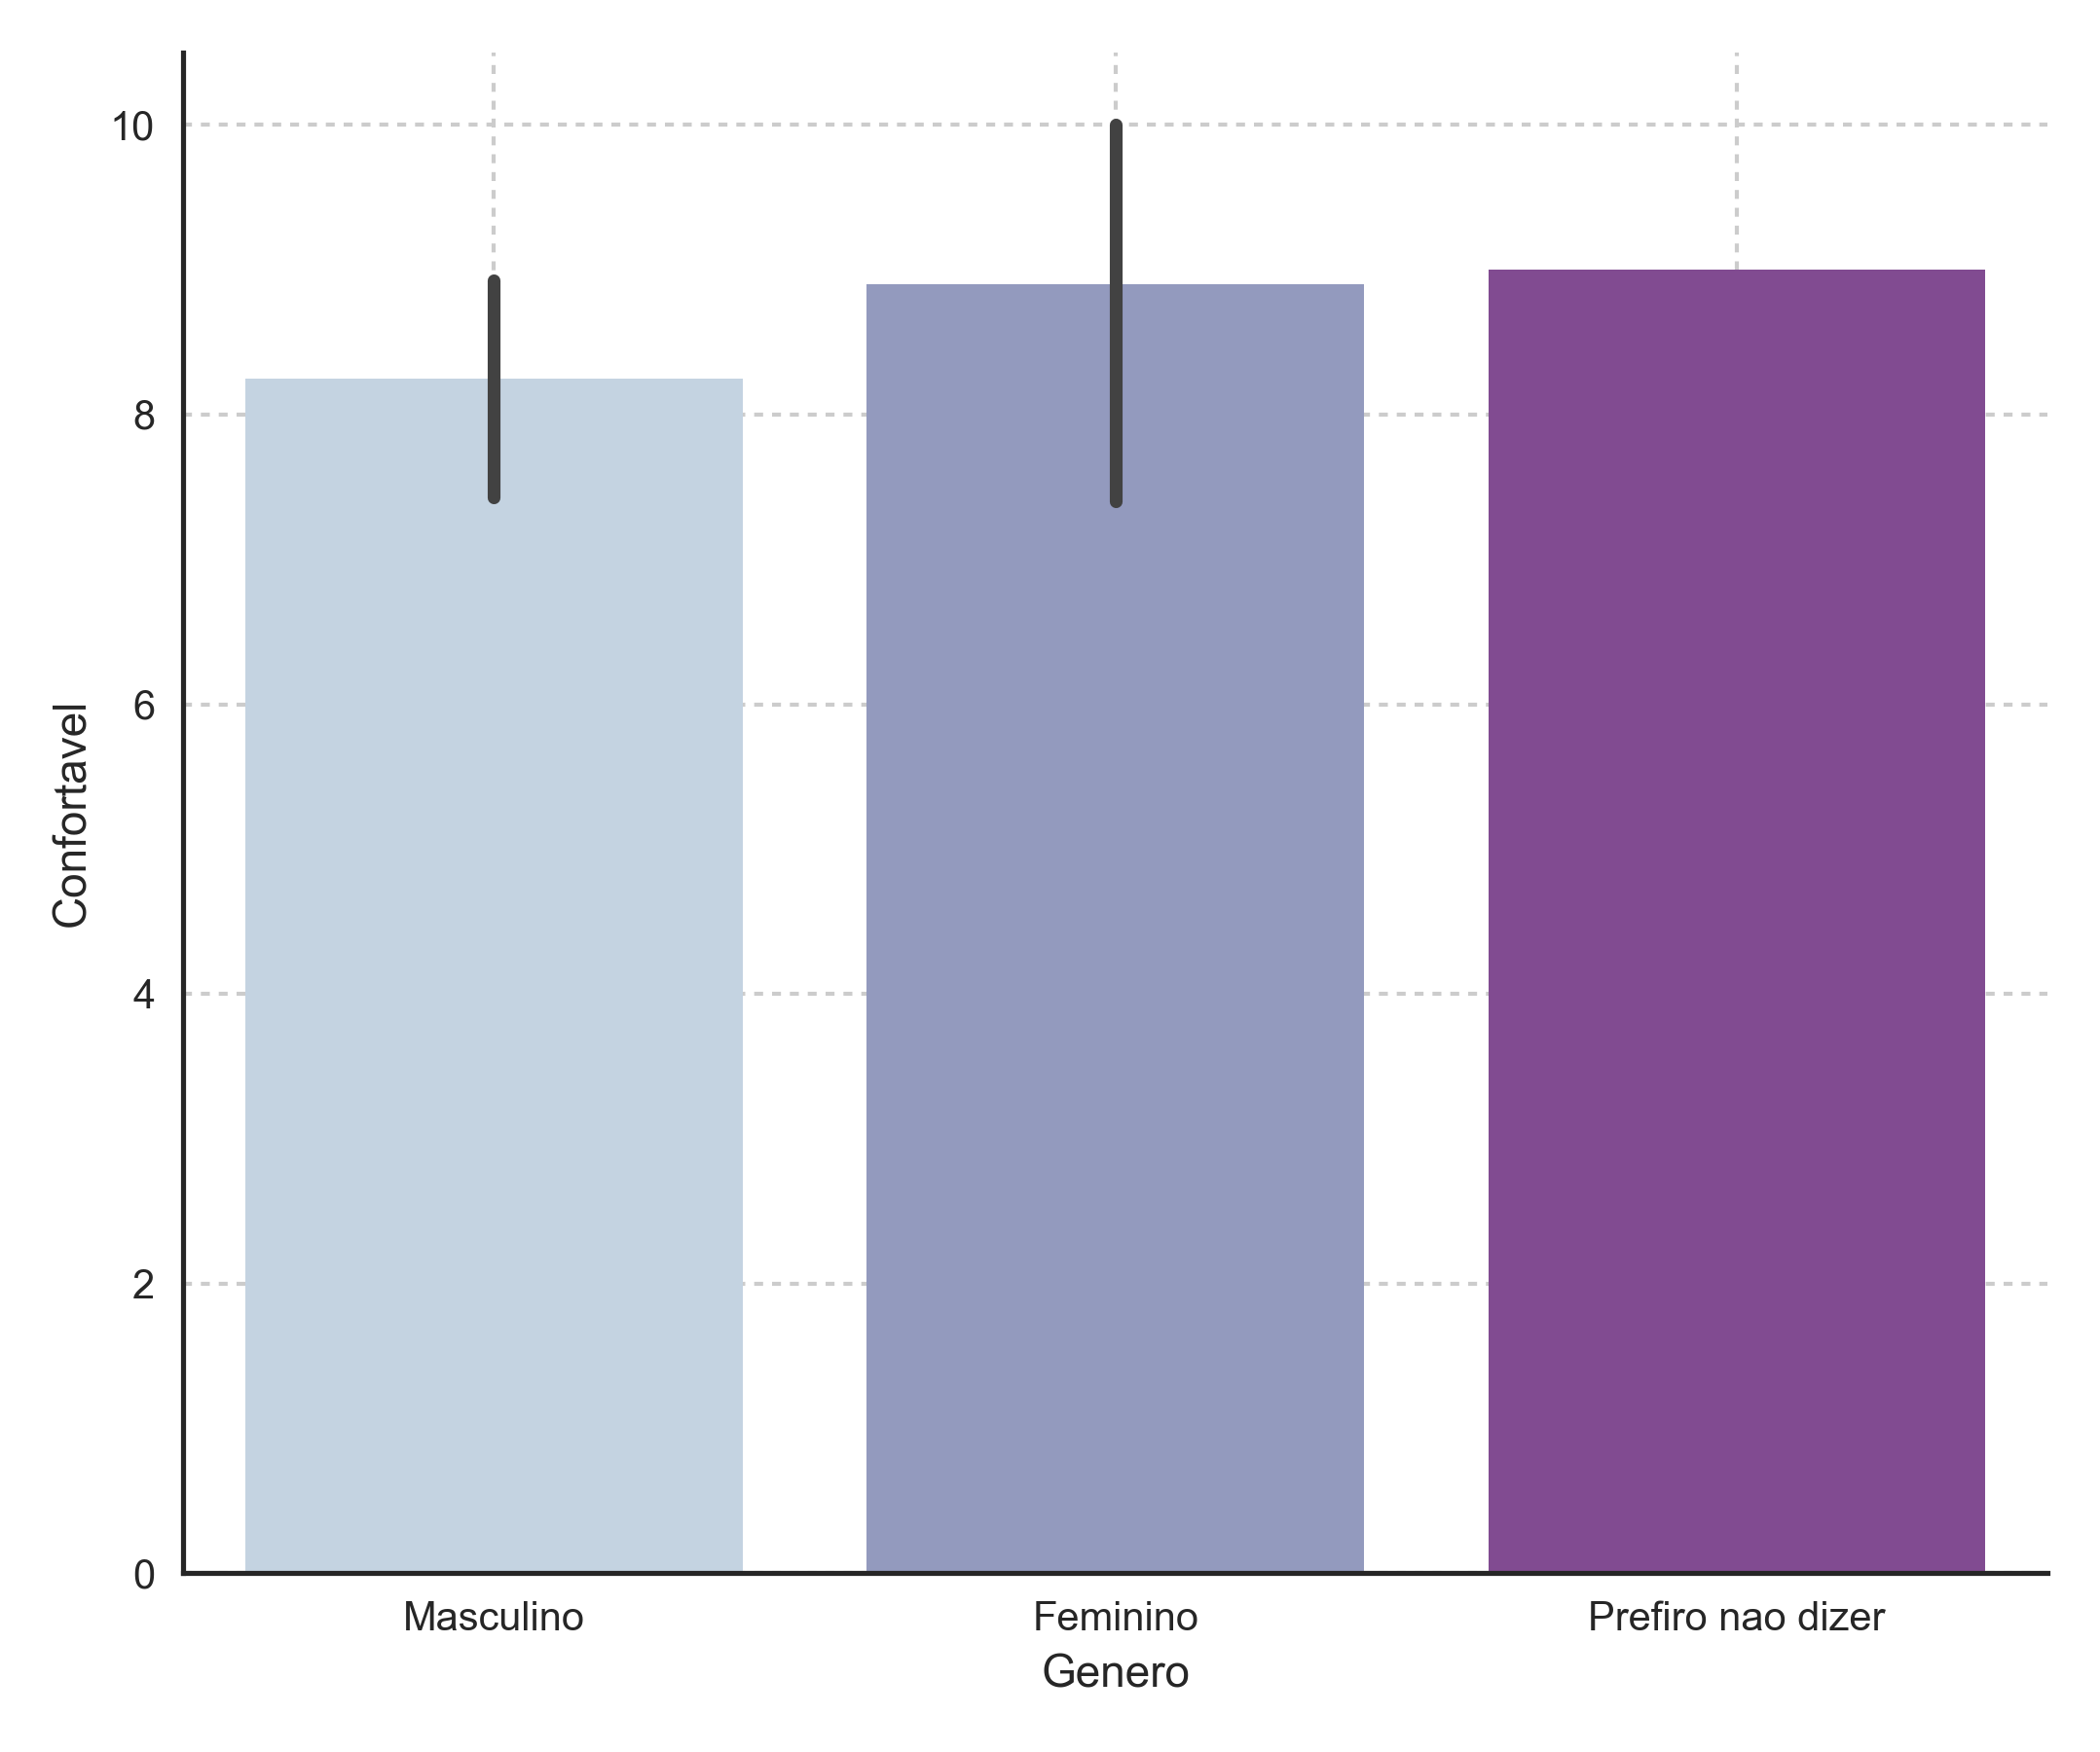
\includegraphics[width=\textwidth]{conforto_genero.png}
		\smallcaption{Fonte: O autor.}
		\label{fig:confortogenero}
	\end{minipage}
\end{figure}

Pode-se observar na figura~\ref{fig:confortogenero} que o gênero que se manteve mais confortável com o robô na aproximação foi o feminino. Isso ocorreu em grande parte devido a exibição das expressões faciais do robô. As participantes do gênero feminino acolheu o robô como uma criança ou pessoa meiga se aproximando dela. Outra variável que é comparada é a idade dos partipantes com o nível de conforto, apresentado na figura~\ref{fig:confortoidade}.

\begin{figure}[ht!]
	\centering
	\begin{minipage}{0.65\textwidth}
		\caption{Conforto por idade.}
		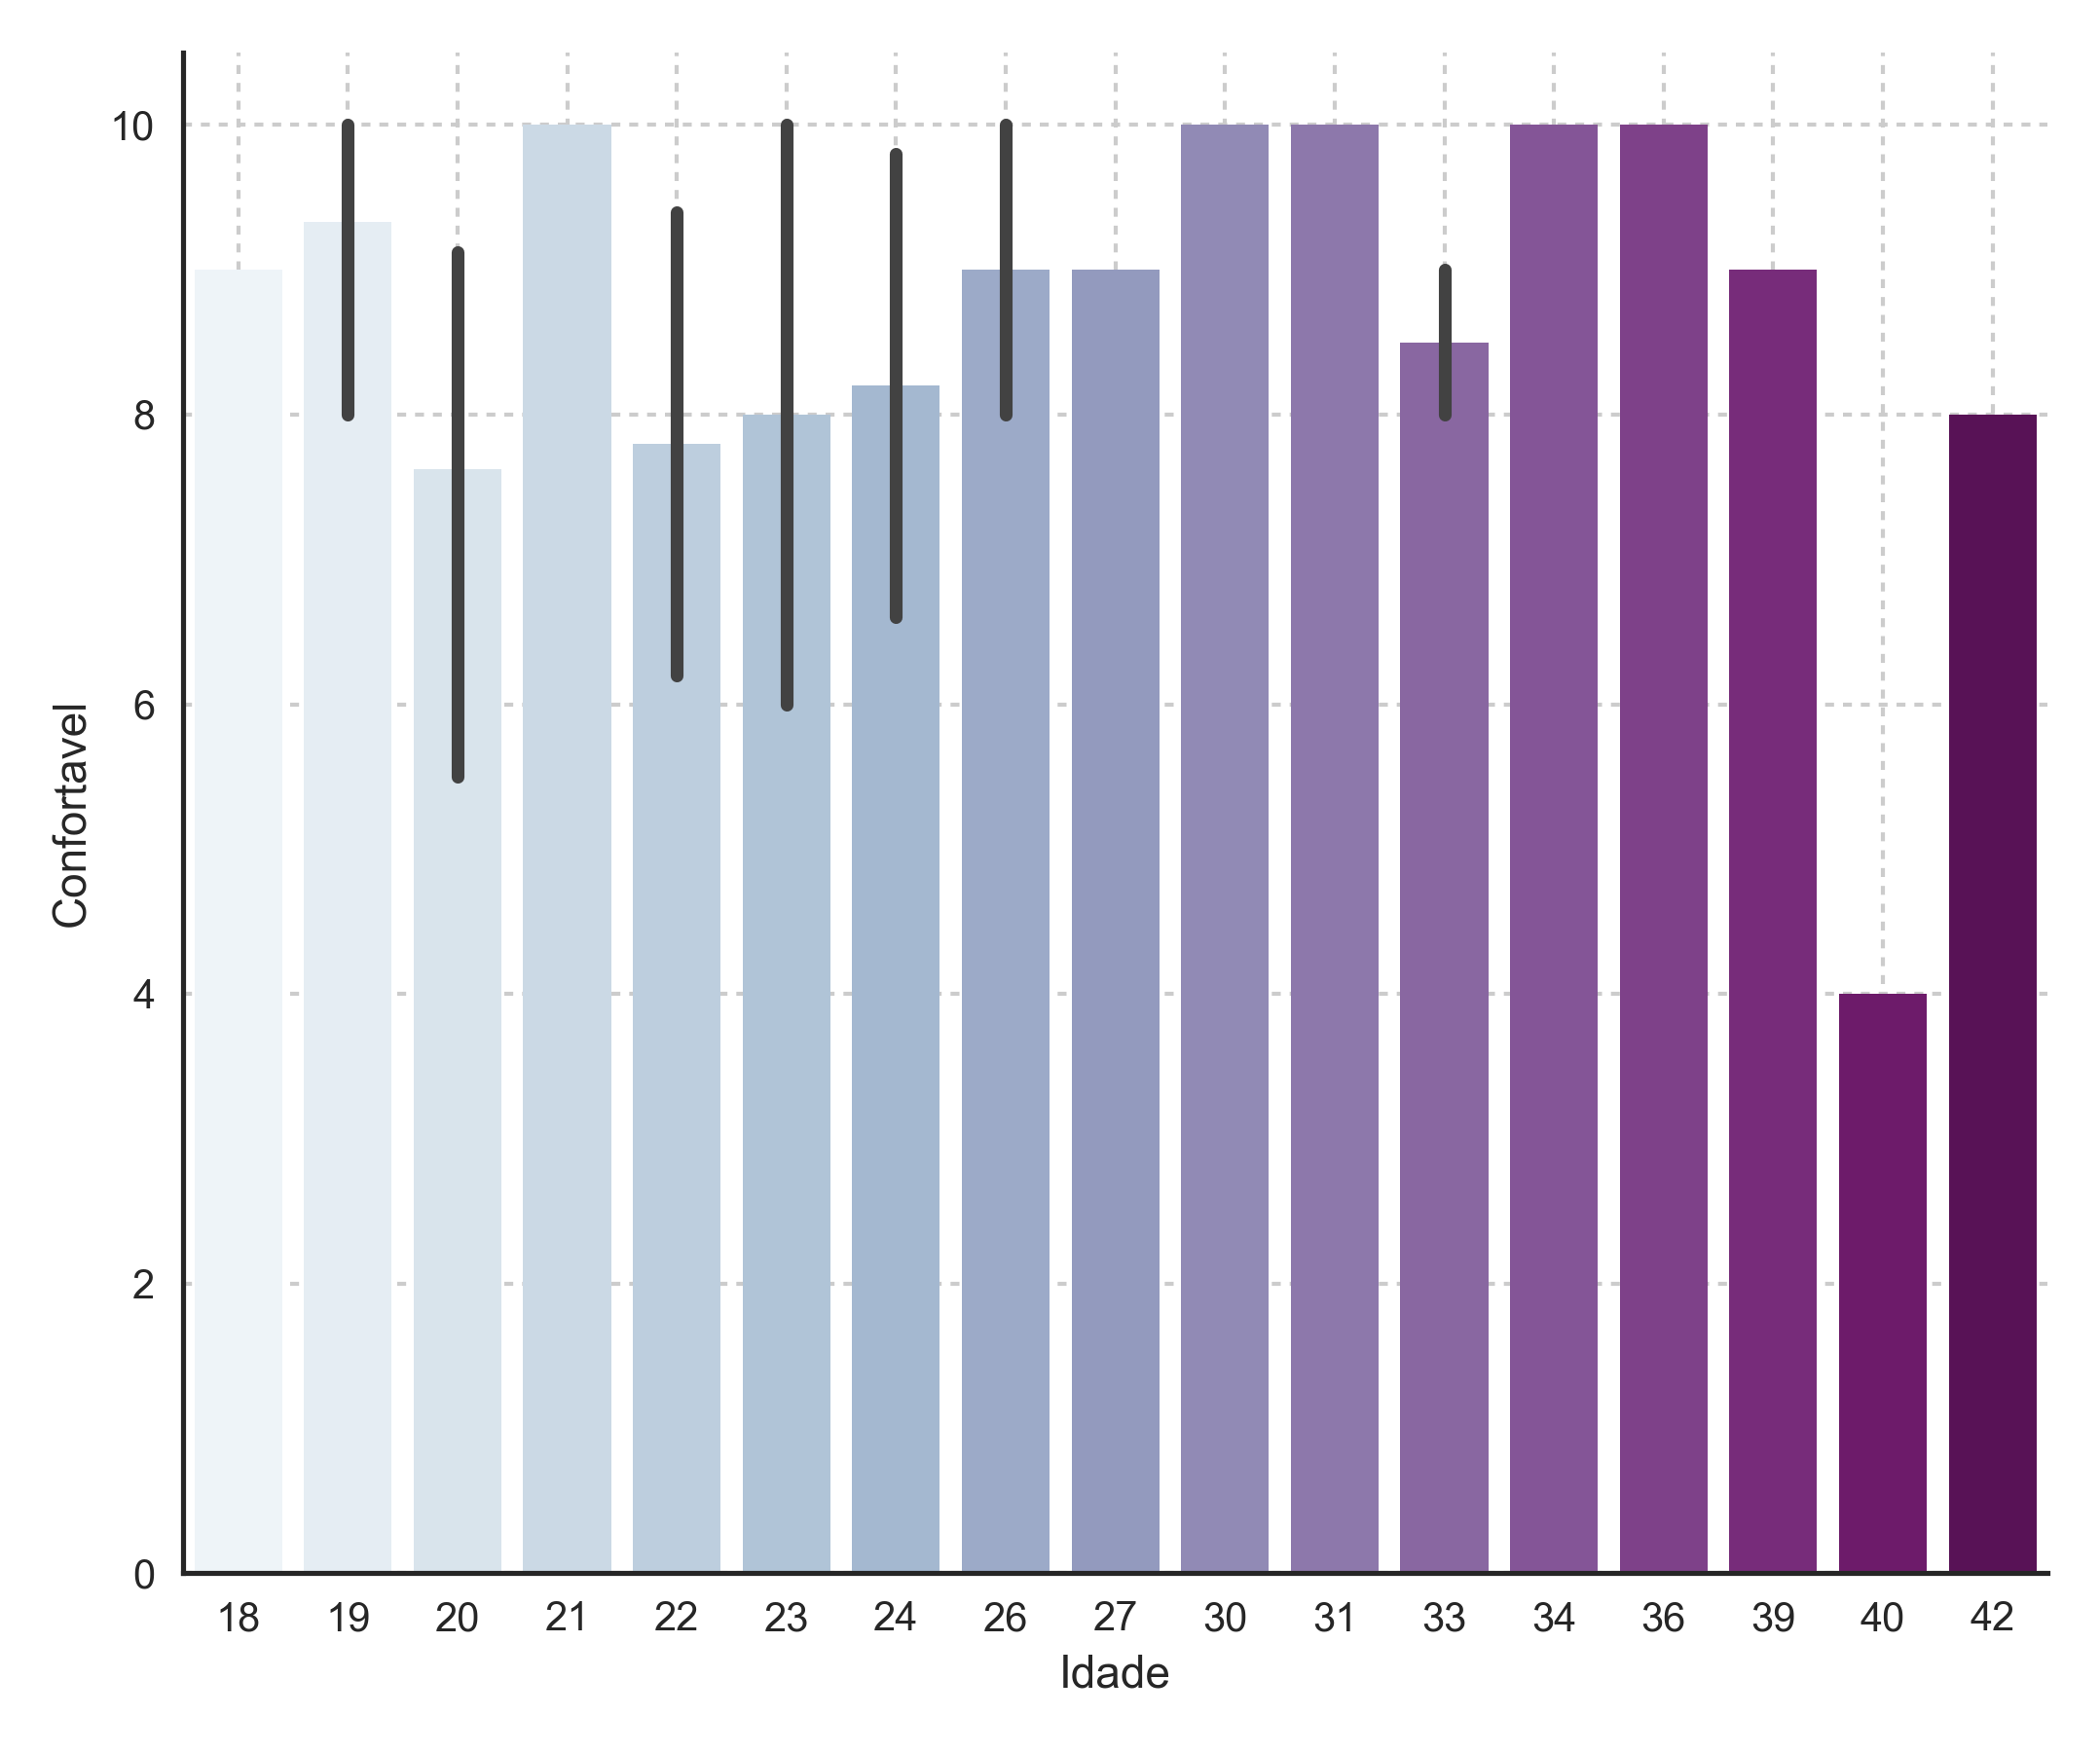
\includegraphics[width=\textwidth]{conforto_idade.png}
		\smallcaption{Fonte: O autor.}
		\label{fig:confortoidade}
	\end{minipage}
\end{figure}

Uma observação interessante é que apenas dois participantes apresentaram um nível de desconforto alto na aproximação do robô. Um participante de 20 e outro de 40 anos ficaram mais desconfortáveis com o robô, como observado na figura~\ref{fig:confortoidade}.

Na figura~\ref{fig:confortoposicao} é apresentada a relação entre o conforto do participante e a posição dele durante a interação, sentado ou em pé.

\begin{figure}[ht!]
	\centering
	\begin{minipage}{0.65\textwidth}
		\caption{Conforto por posição de interação.}
		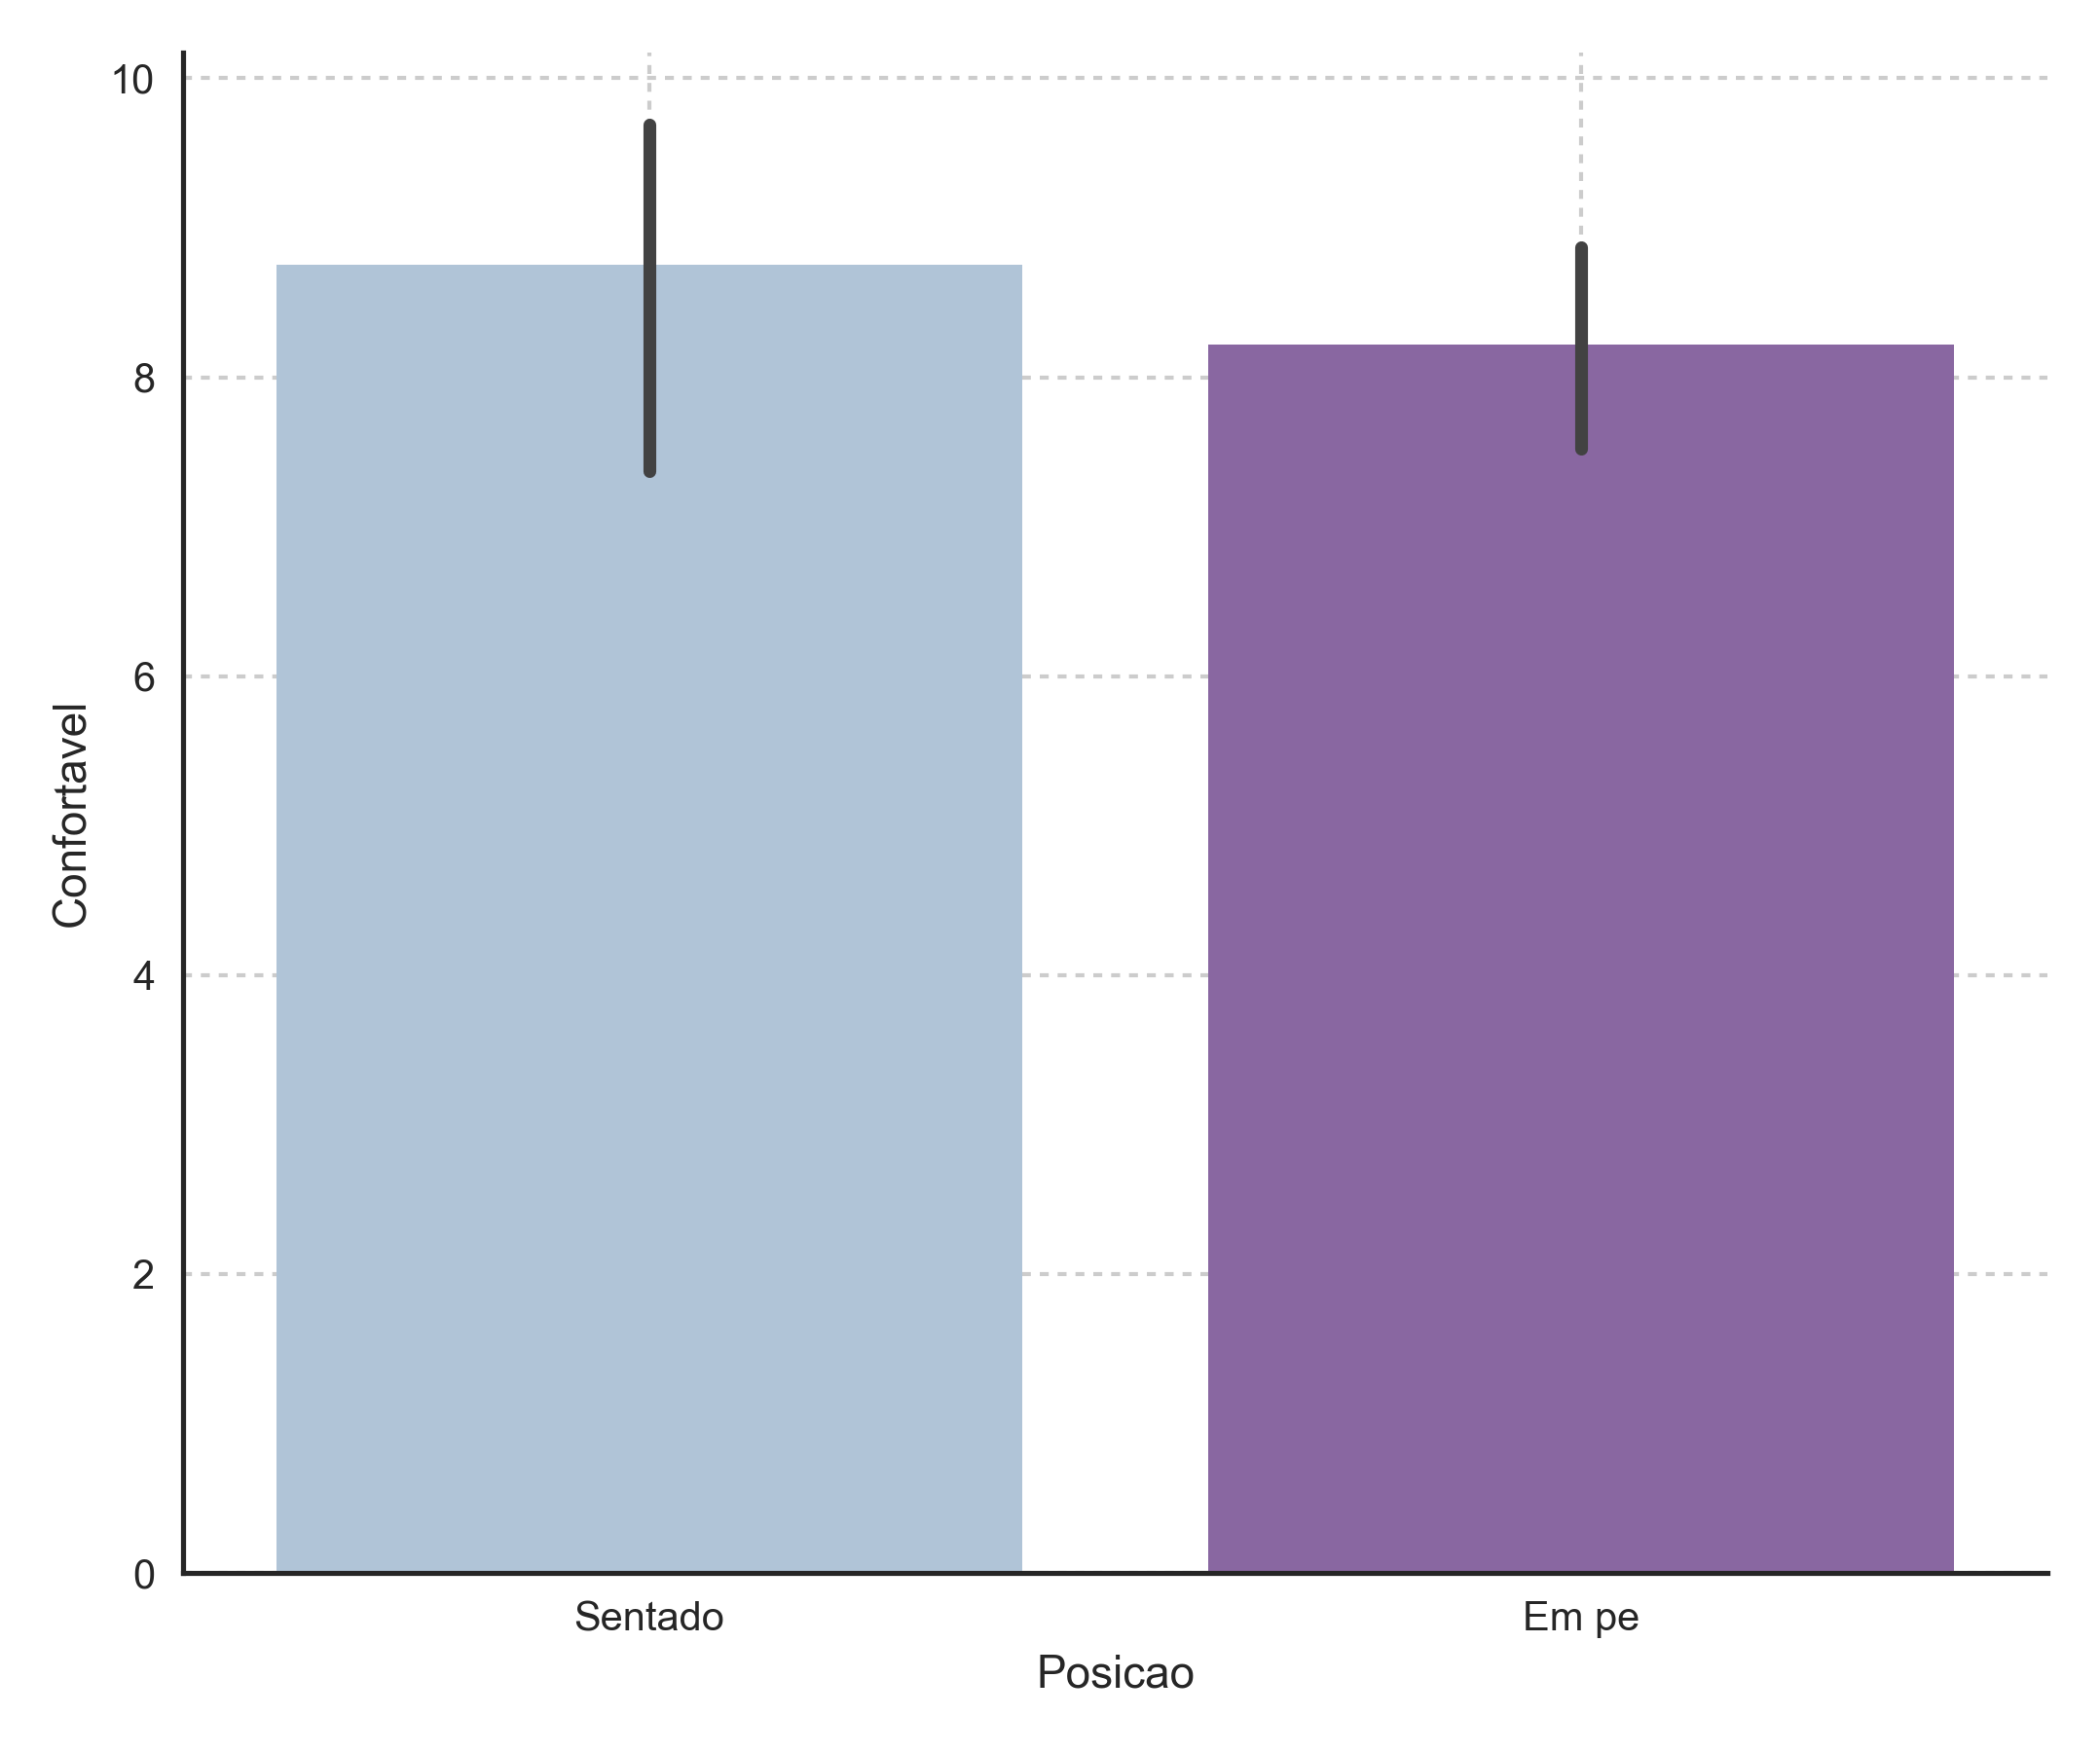
\includegraphics[width=\textwidth]{conforto_posicao.png}
		\smallcaption{Fonte: O autor.}
		\label{fig:confortoposicao}
	\end{minipage}
\end{figure}

É observado na figura~\ref{fig:confortoposicao} algo que foi observado diferente na competição da RoboCup, onde as pessoas sentadas sentiram maior desconforto. Nos testes, as pessoas que estavam sentadas durante a interação com o robô sentiram-se mais confortavéis do que as pessoas que estavam em pé. Esse é um fenômeno que pode ocorrer, pois o robô tocou no braço e barriga de alguns participantes que estavam em pé quando esticou o manipulador para chamar a atenção deles. Por último, é apresentado na figura~\ref{fig:confortosociavel} o nível de conforto dos participantes, dado a sua declaração de sociável ou não.

\begin{figure}[ht!]
	\centering
	\begin{minipage}{0.65\textwidth}
		\caption{Conforto por declaração de sociável.}
		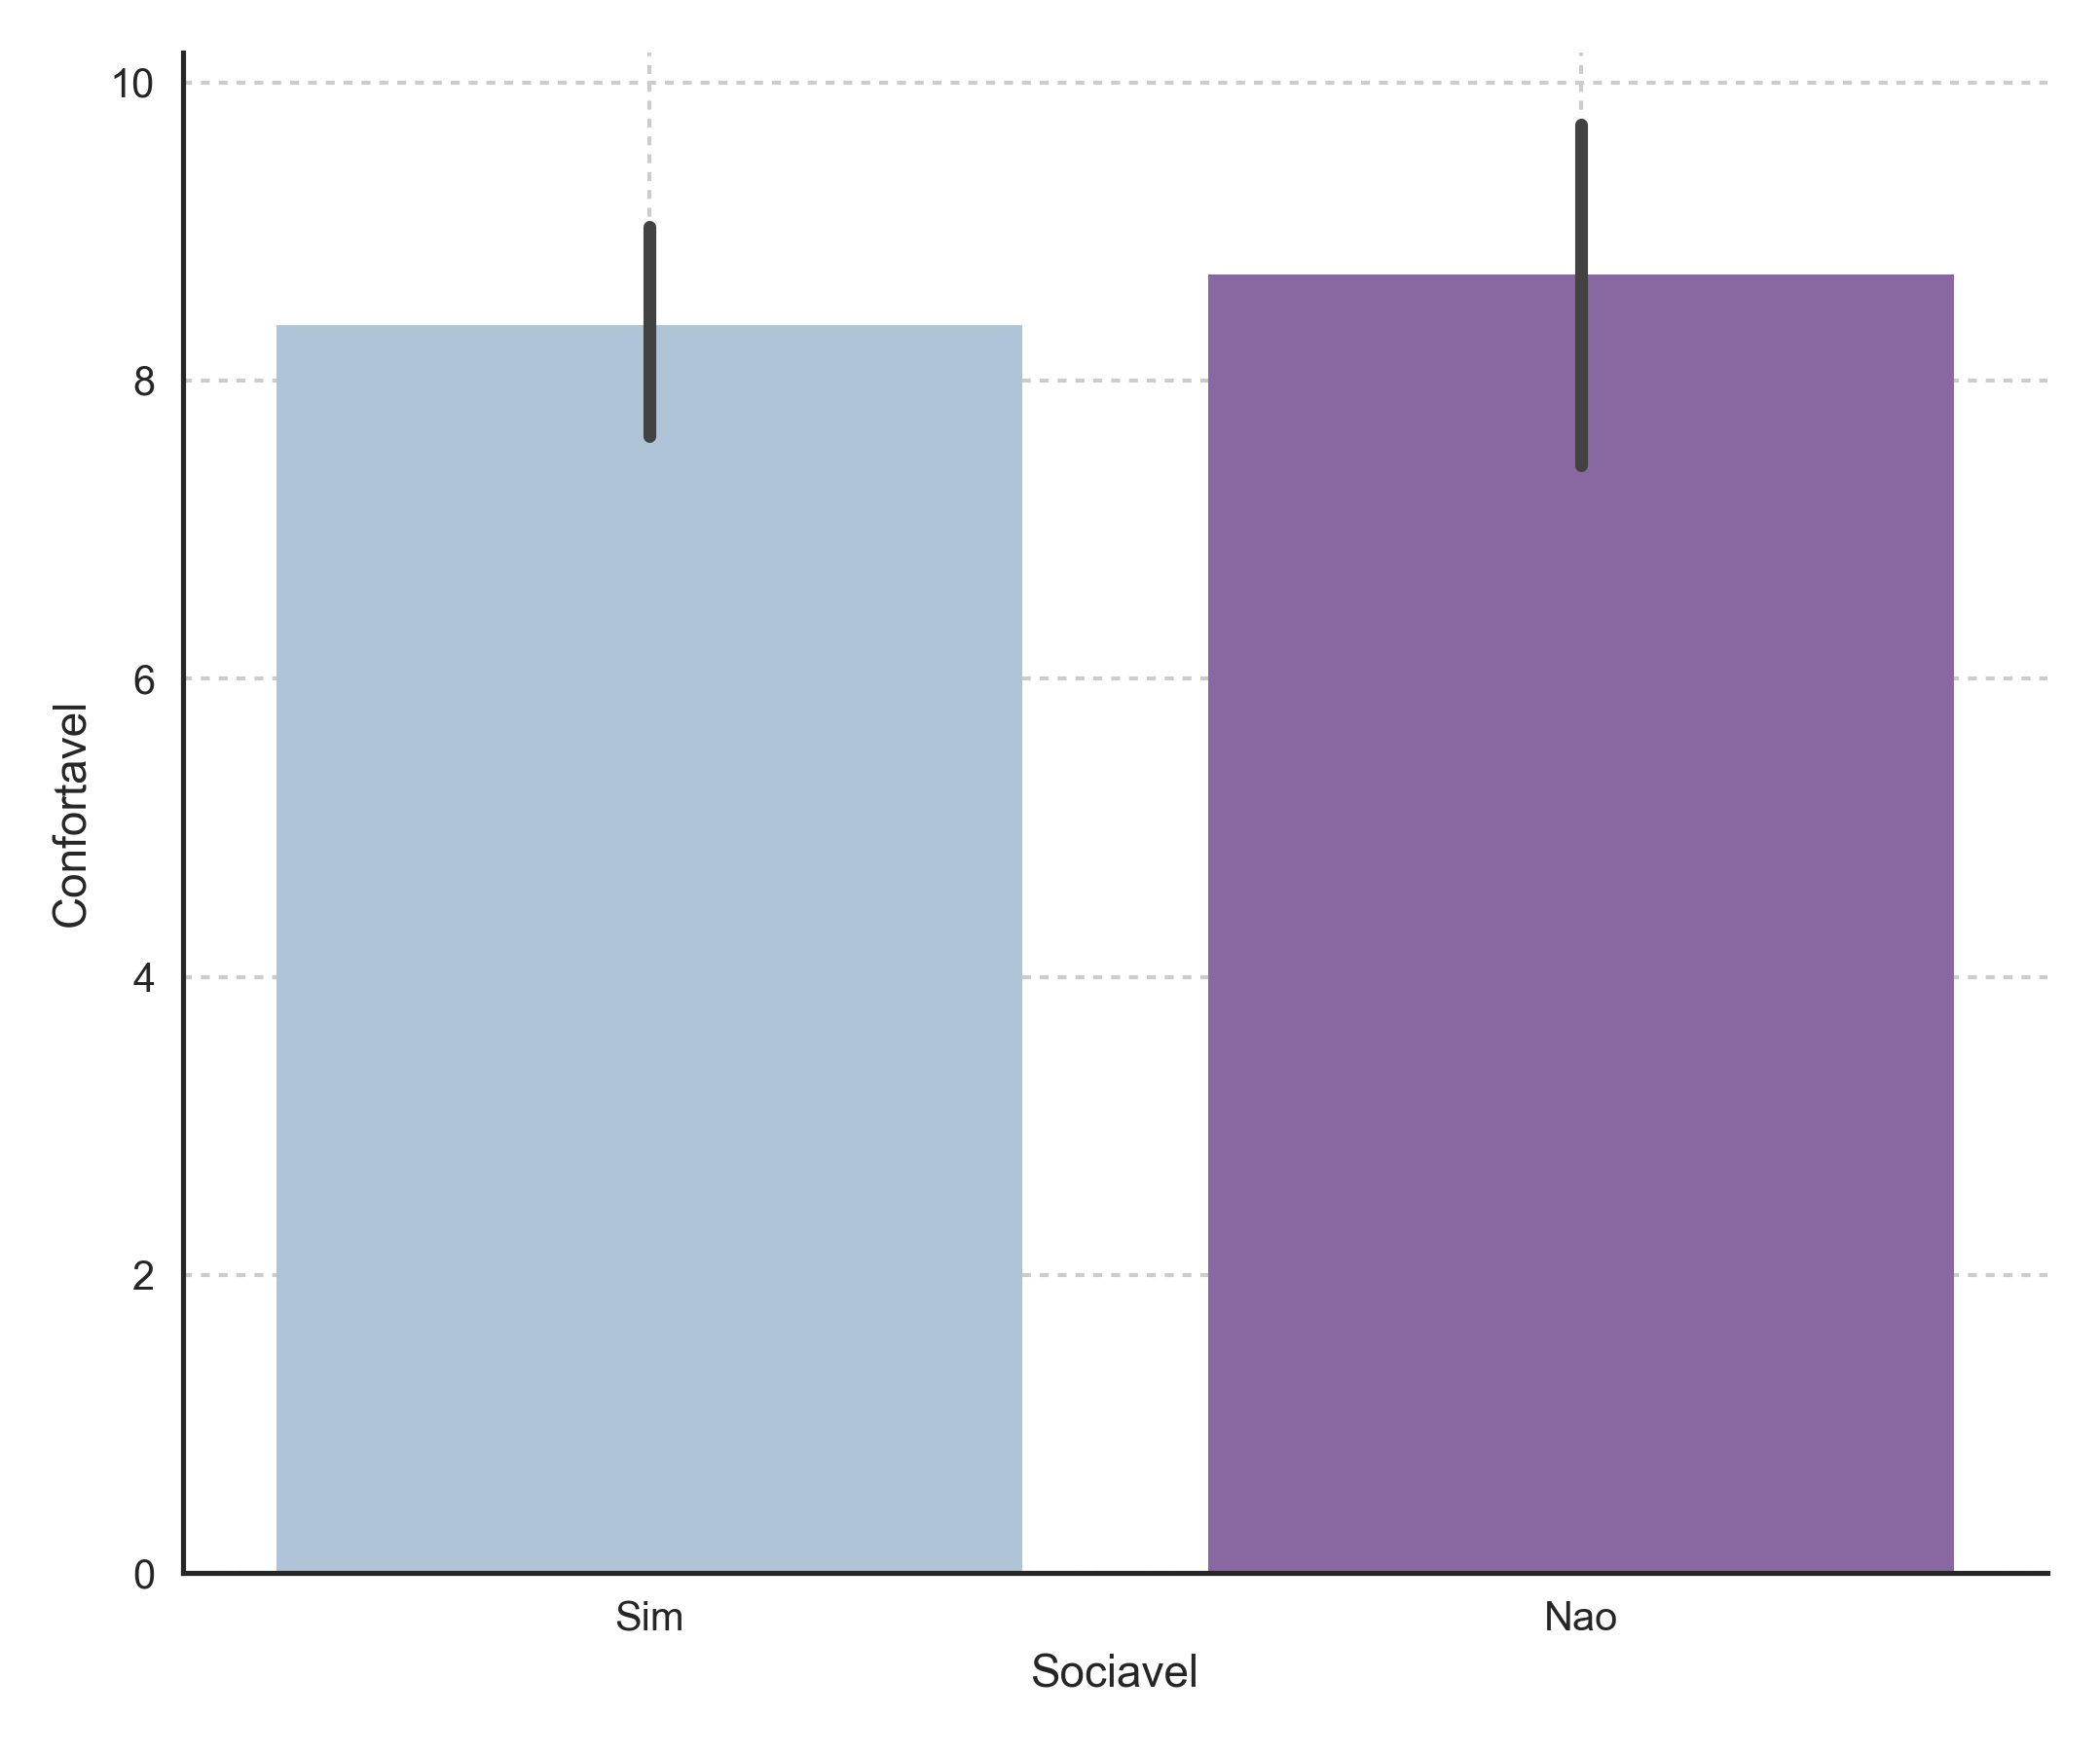
\includegraphics[width=\textwidth]{conforto_sociavel.png}
		\smallcaption{Fonte: O autor.}
		\label{fig:confortosociavel}
	\end{minipage}
\end{figure}

Mais um ponto interessante nessa análise feita através da figura~\ref{fig:confortosocial}. As pessoas declaradas como não sociáveis, foram as pessoas que mais se sentiram confortáveis durante toda a aproximação do robô. É um ponto interessante, pois se observar pela lógica, as pessoas sociáveis deveriam estar mais confortável e abertas a novas experiências.

A mesma análise para o conforto do usuário, foi realizada para a declaração de medo. Na escala da pergunta de medo o menor valor corresponde a totalmente com medo e o maior corresponde a totalmente sem medo. A figura~\ref{fig:medogenero} apresenta a relação entre o medo e o gênero do participante.

\begin{figure}[ht!]
	\centering
	\begin{minipage}{0.65\textwidth}
		\caption{Medo por gênero.}
		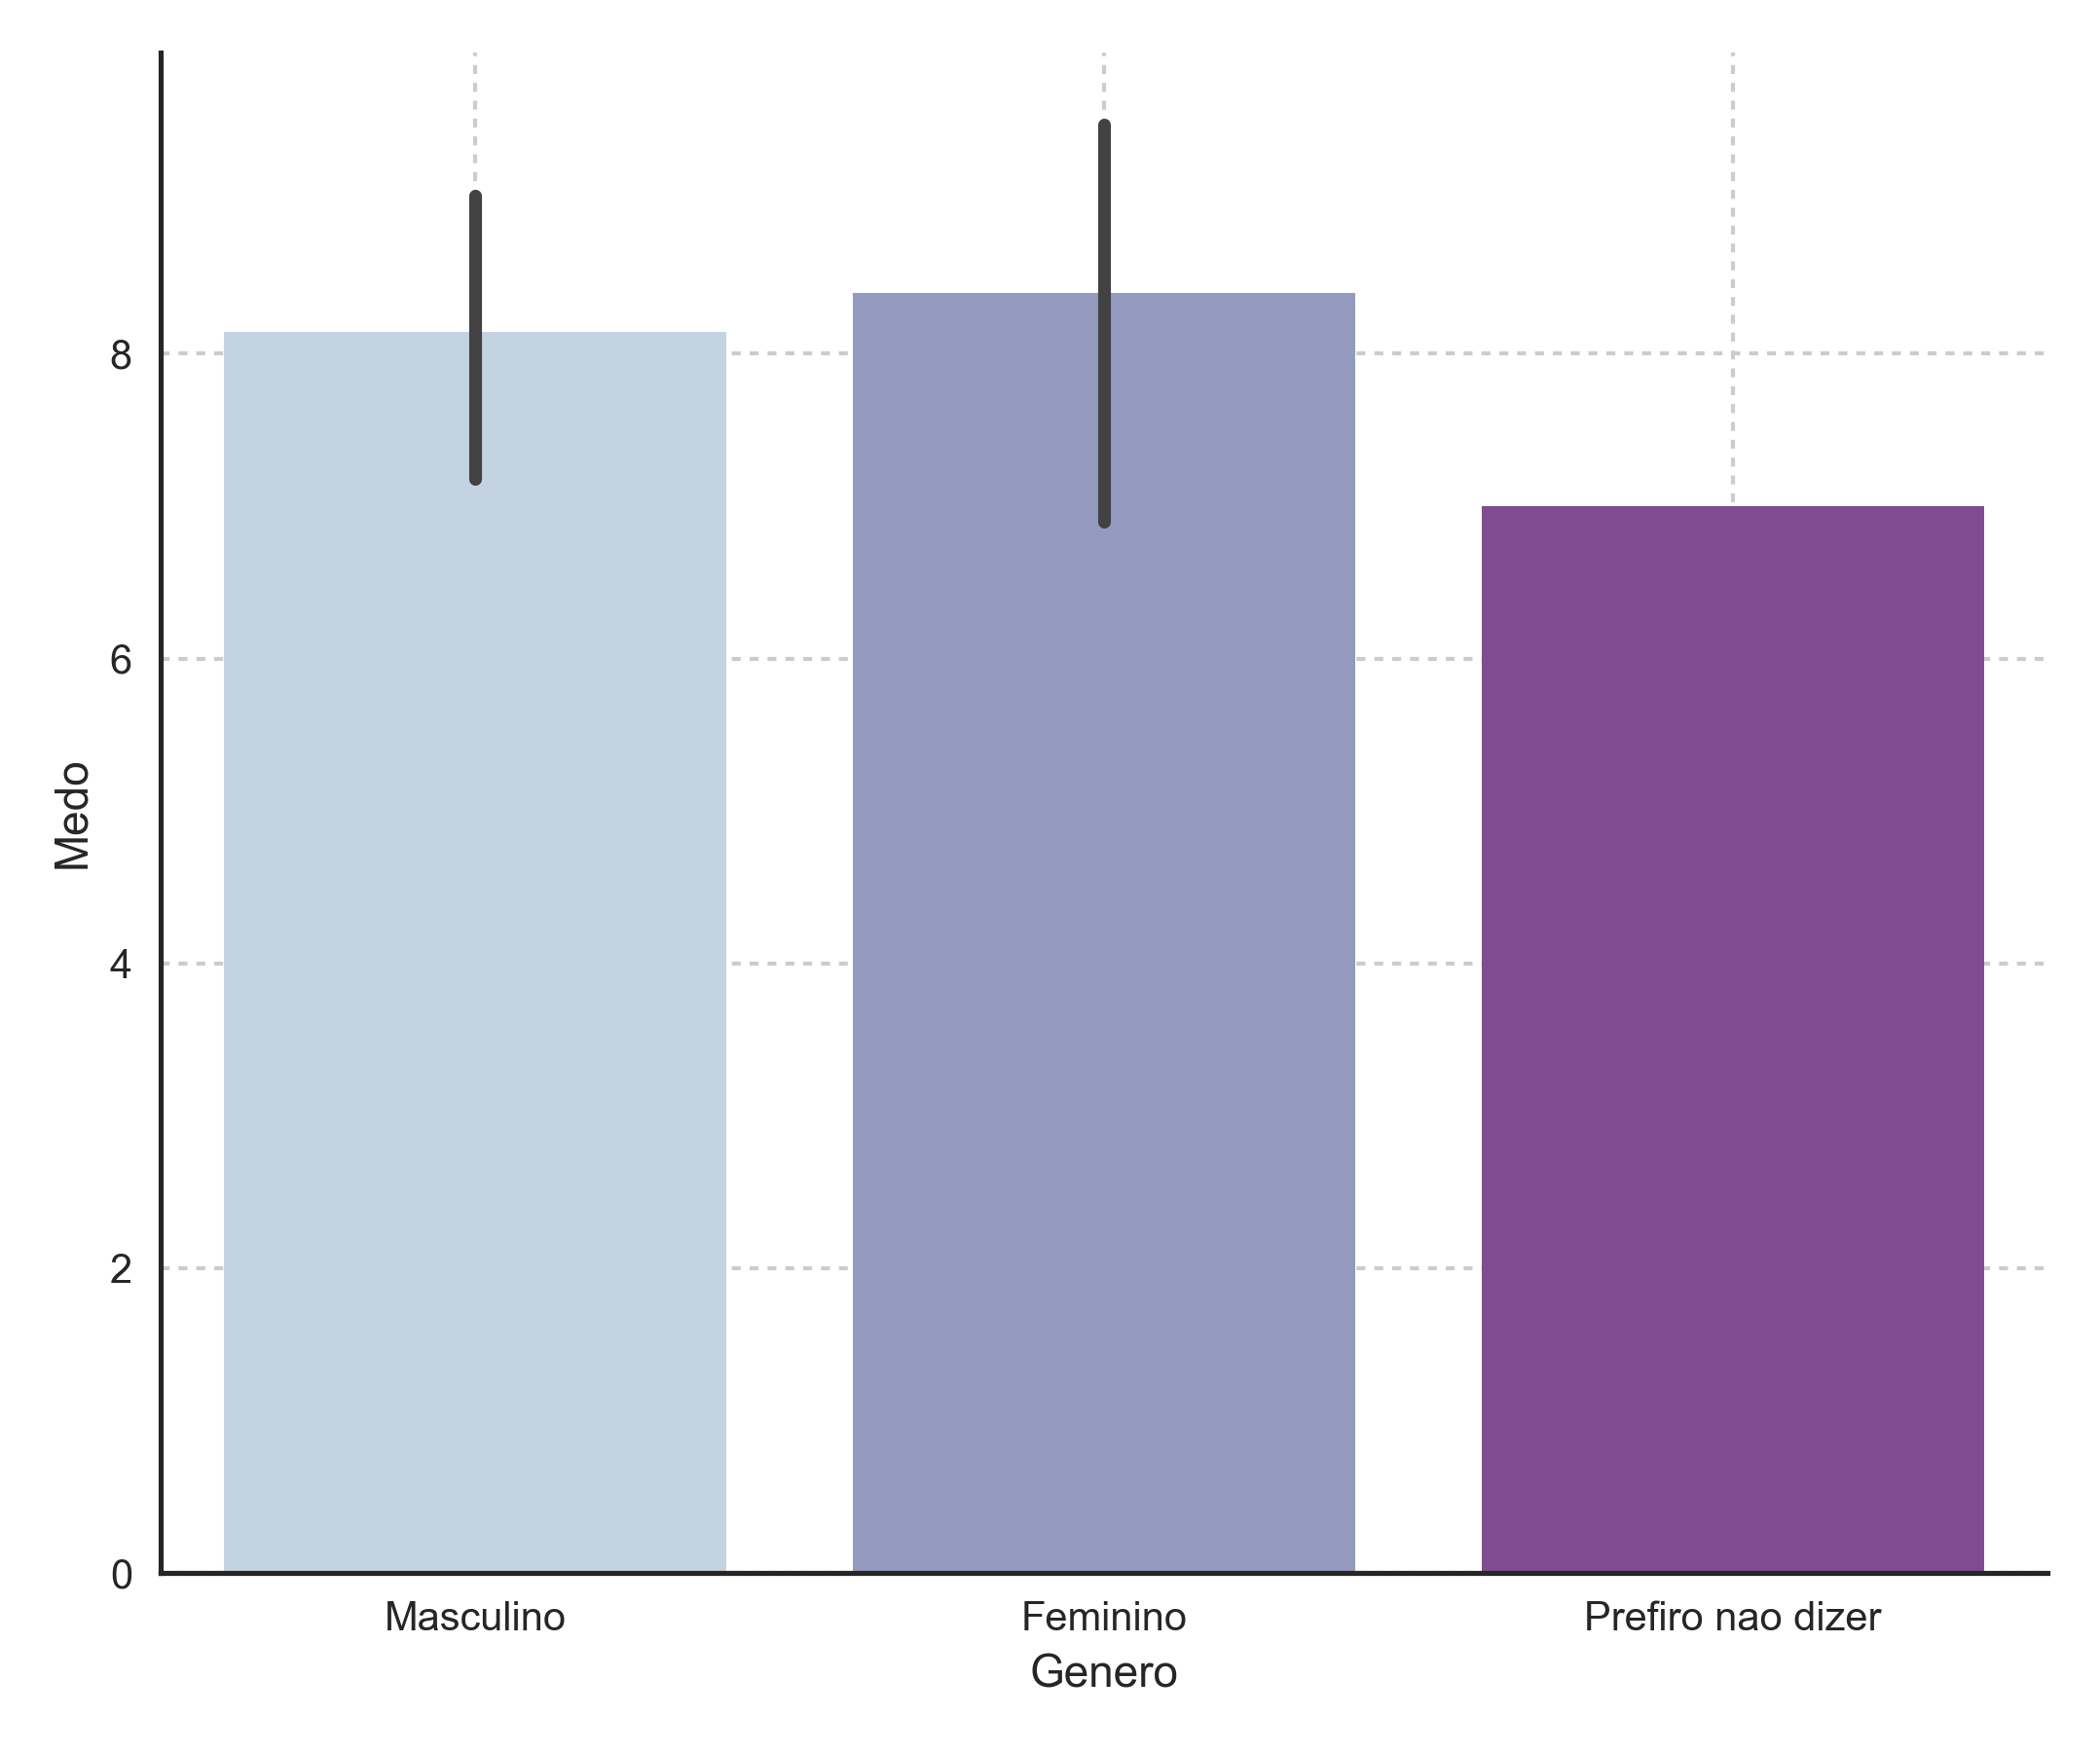
\includegraphics[width=\textwidth]{medo_genero.png}
		\smallcaption{Fonte: O autor.}
		\label{fig:medogenero}
	\end{minipage}
\end{figure}

Para a relação de medo e gênero, o que demonstrou menos medo foi o feminino. Isso era esperado devido ao resultado obtido sobre o conforto do usuário, apesar de nem sempre essa relação ser diretamente proporcional. A próxima análise é realizada com base na relação medo e idade, como demonstra a figura~\ref{fig:medoidade}.

\begin{figure}[ht!]
	\centering
	\begin{minipage}{0.65\textwidth}
		\caption{Medo por idade.}
		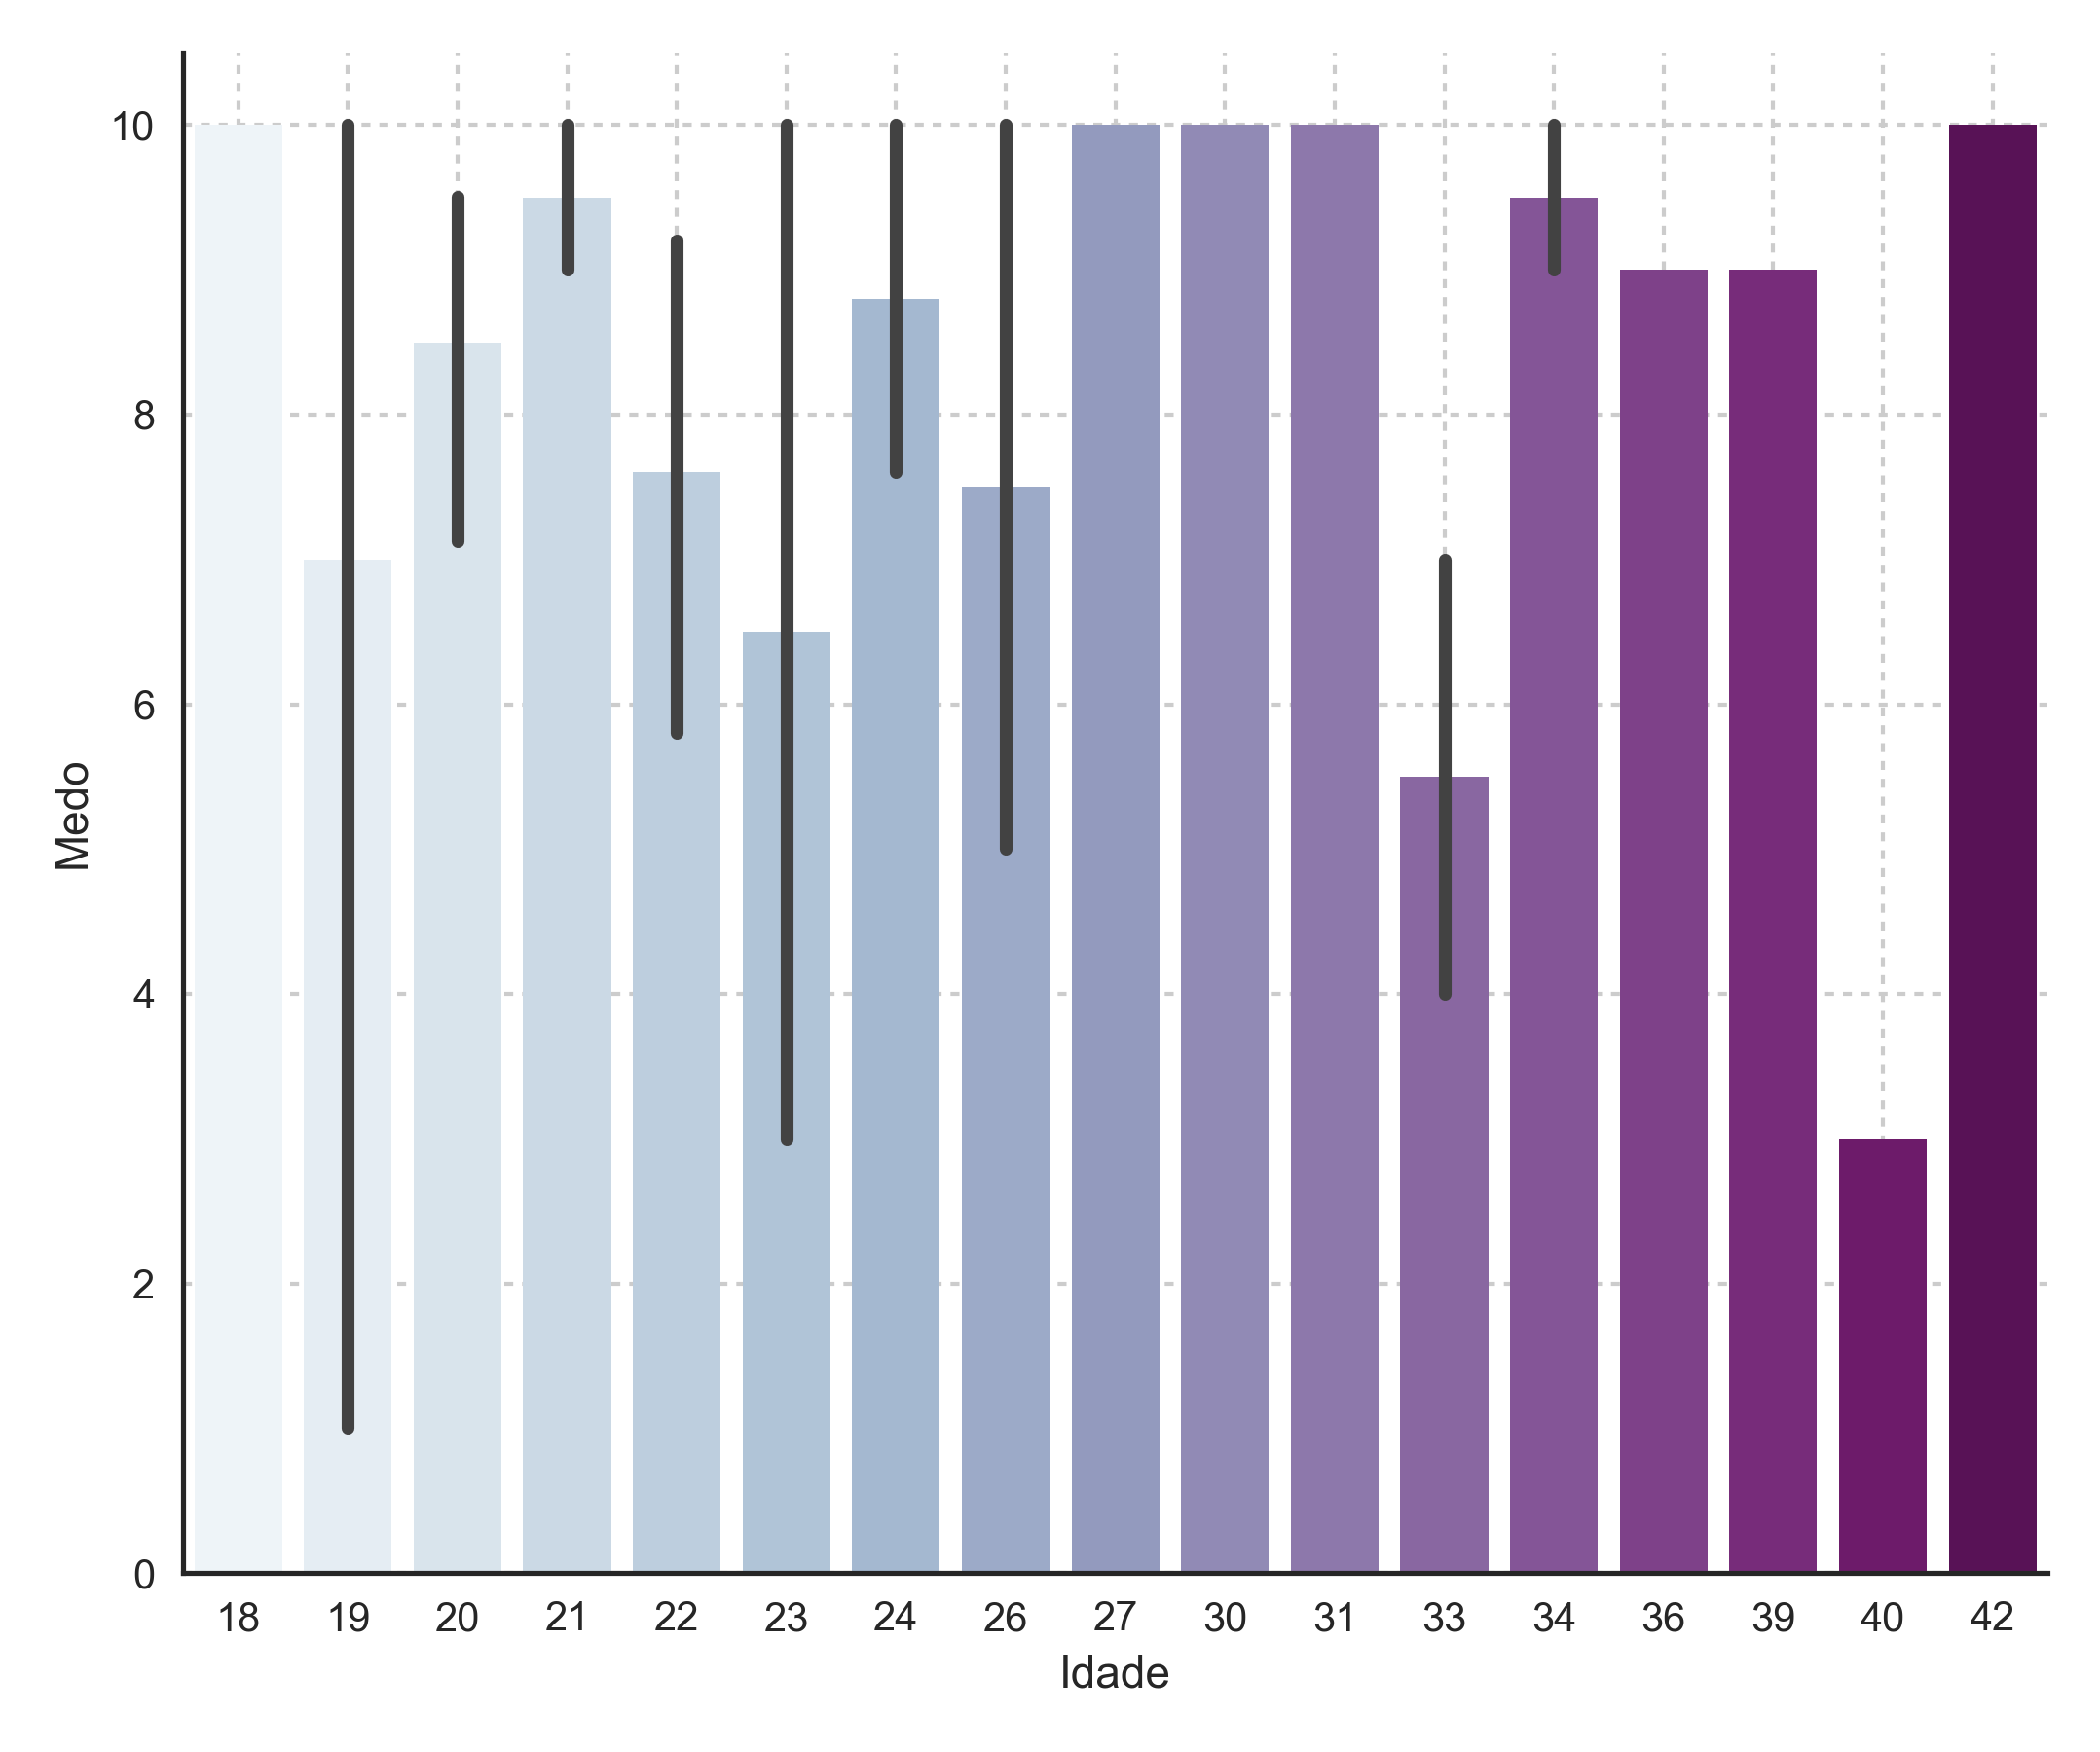
\includegraphics[width=\textwidth]{medo_idade.png}
		\smallcaption{Fonte: O autor.}
		\label{fig:medoidade}
	\end{minipage}
\end{figure}

A faixa etária com maior índice de medo foi a dos 40 anos de idade. Os participantes com 19 anos também apresentam um índice baixo sobre o medo do participante. Isso ocorreu, pois com o comportamento invasivo do robô ao aproximar, a garra deixou o participante assustado. Outro ponto levantado foi que o robô ao se movimentar faz muito barulhento.

A figura~\ref{fig:medoposicao} compara a relação do medo declarado do usuário contra a posição dele durante a navegação do robô.

\begin{figure}[ht!]
	\centering
	\begin{minipage}{0.65\textwidth}
		\caption{Medo por posição de interação.}
		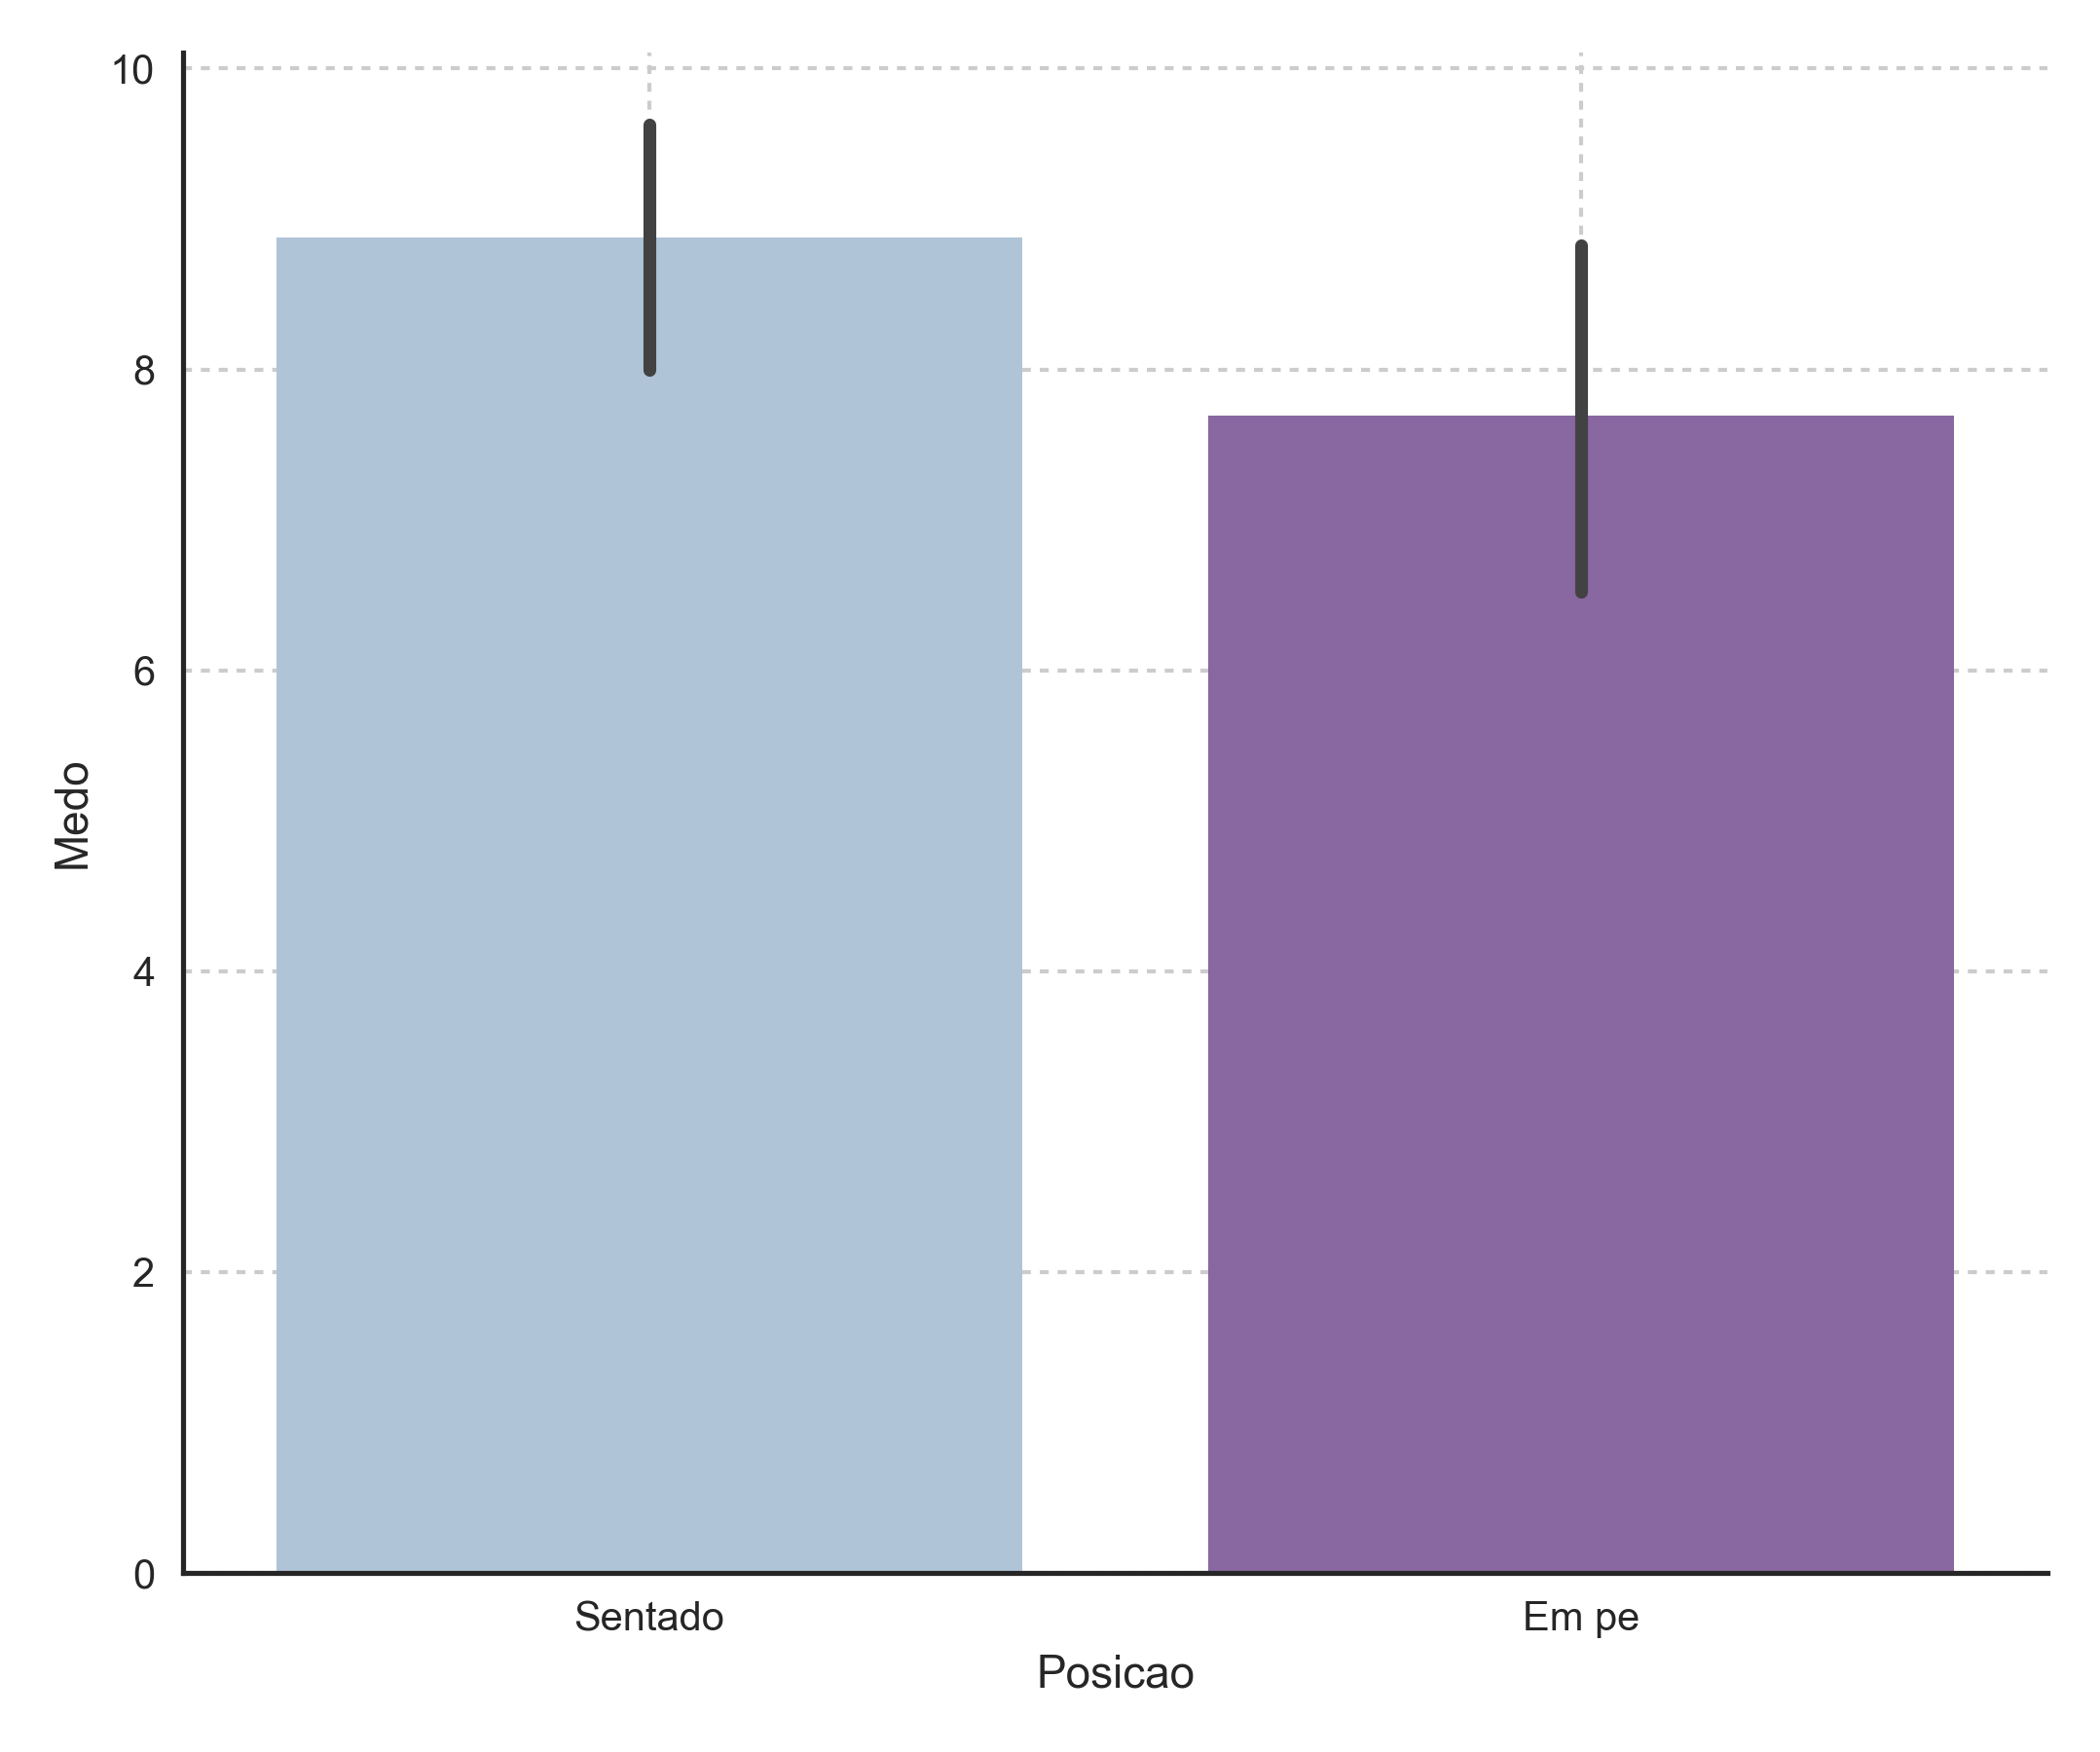
\includegraphics[width=\textwidth]{medo_posicao.png}
		\smallcaption{Fonte: O autor.}
		\label{fig:medoposicao}
	\end{minipage}
\end{figure}

Assim como em relação ao conforto do usuário, os participantes que sentiram mais medo do robô estavam em pé. O manipulador é um ponto de atenção na interação, principalmente quando está dentro do espaço social da pessoa. Os maiores índices de medo ocorreram por que o robô encostou o manipulador na pessoa. As pessoas mais sociáveis sentiram menos medo que as menos sociáveis, como apresenta na figura~\ref{fig:medosociavel}.

\begin{figure}[ht!]
	\centering
	\begin{minipage}{0.65\textwidth}
		\caption{Medo por declaração de sociável.}
		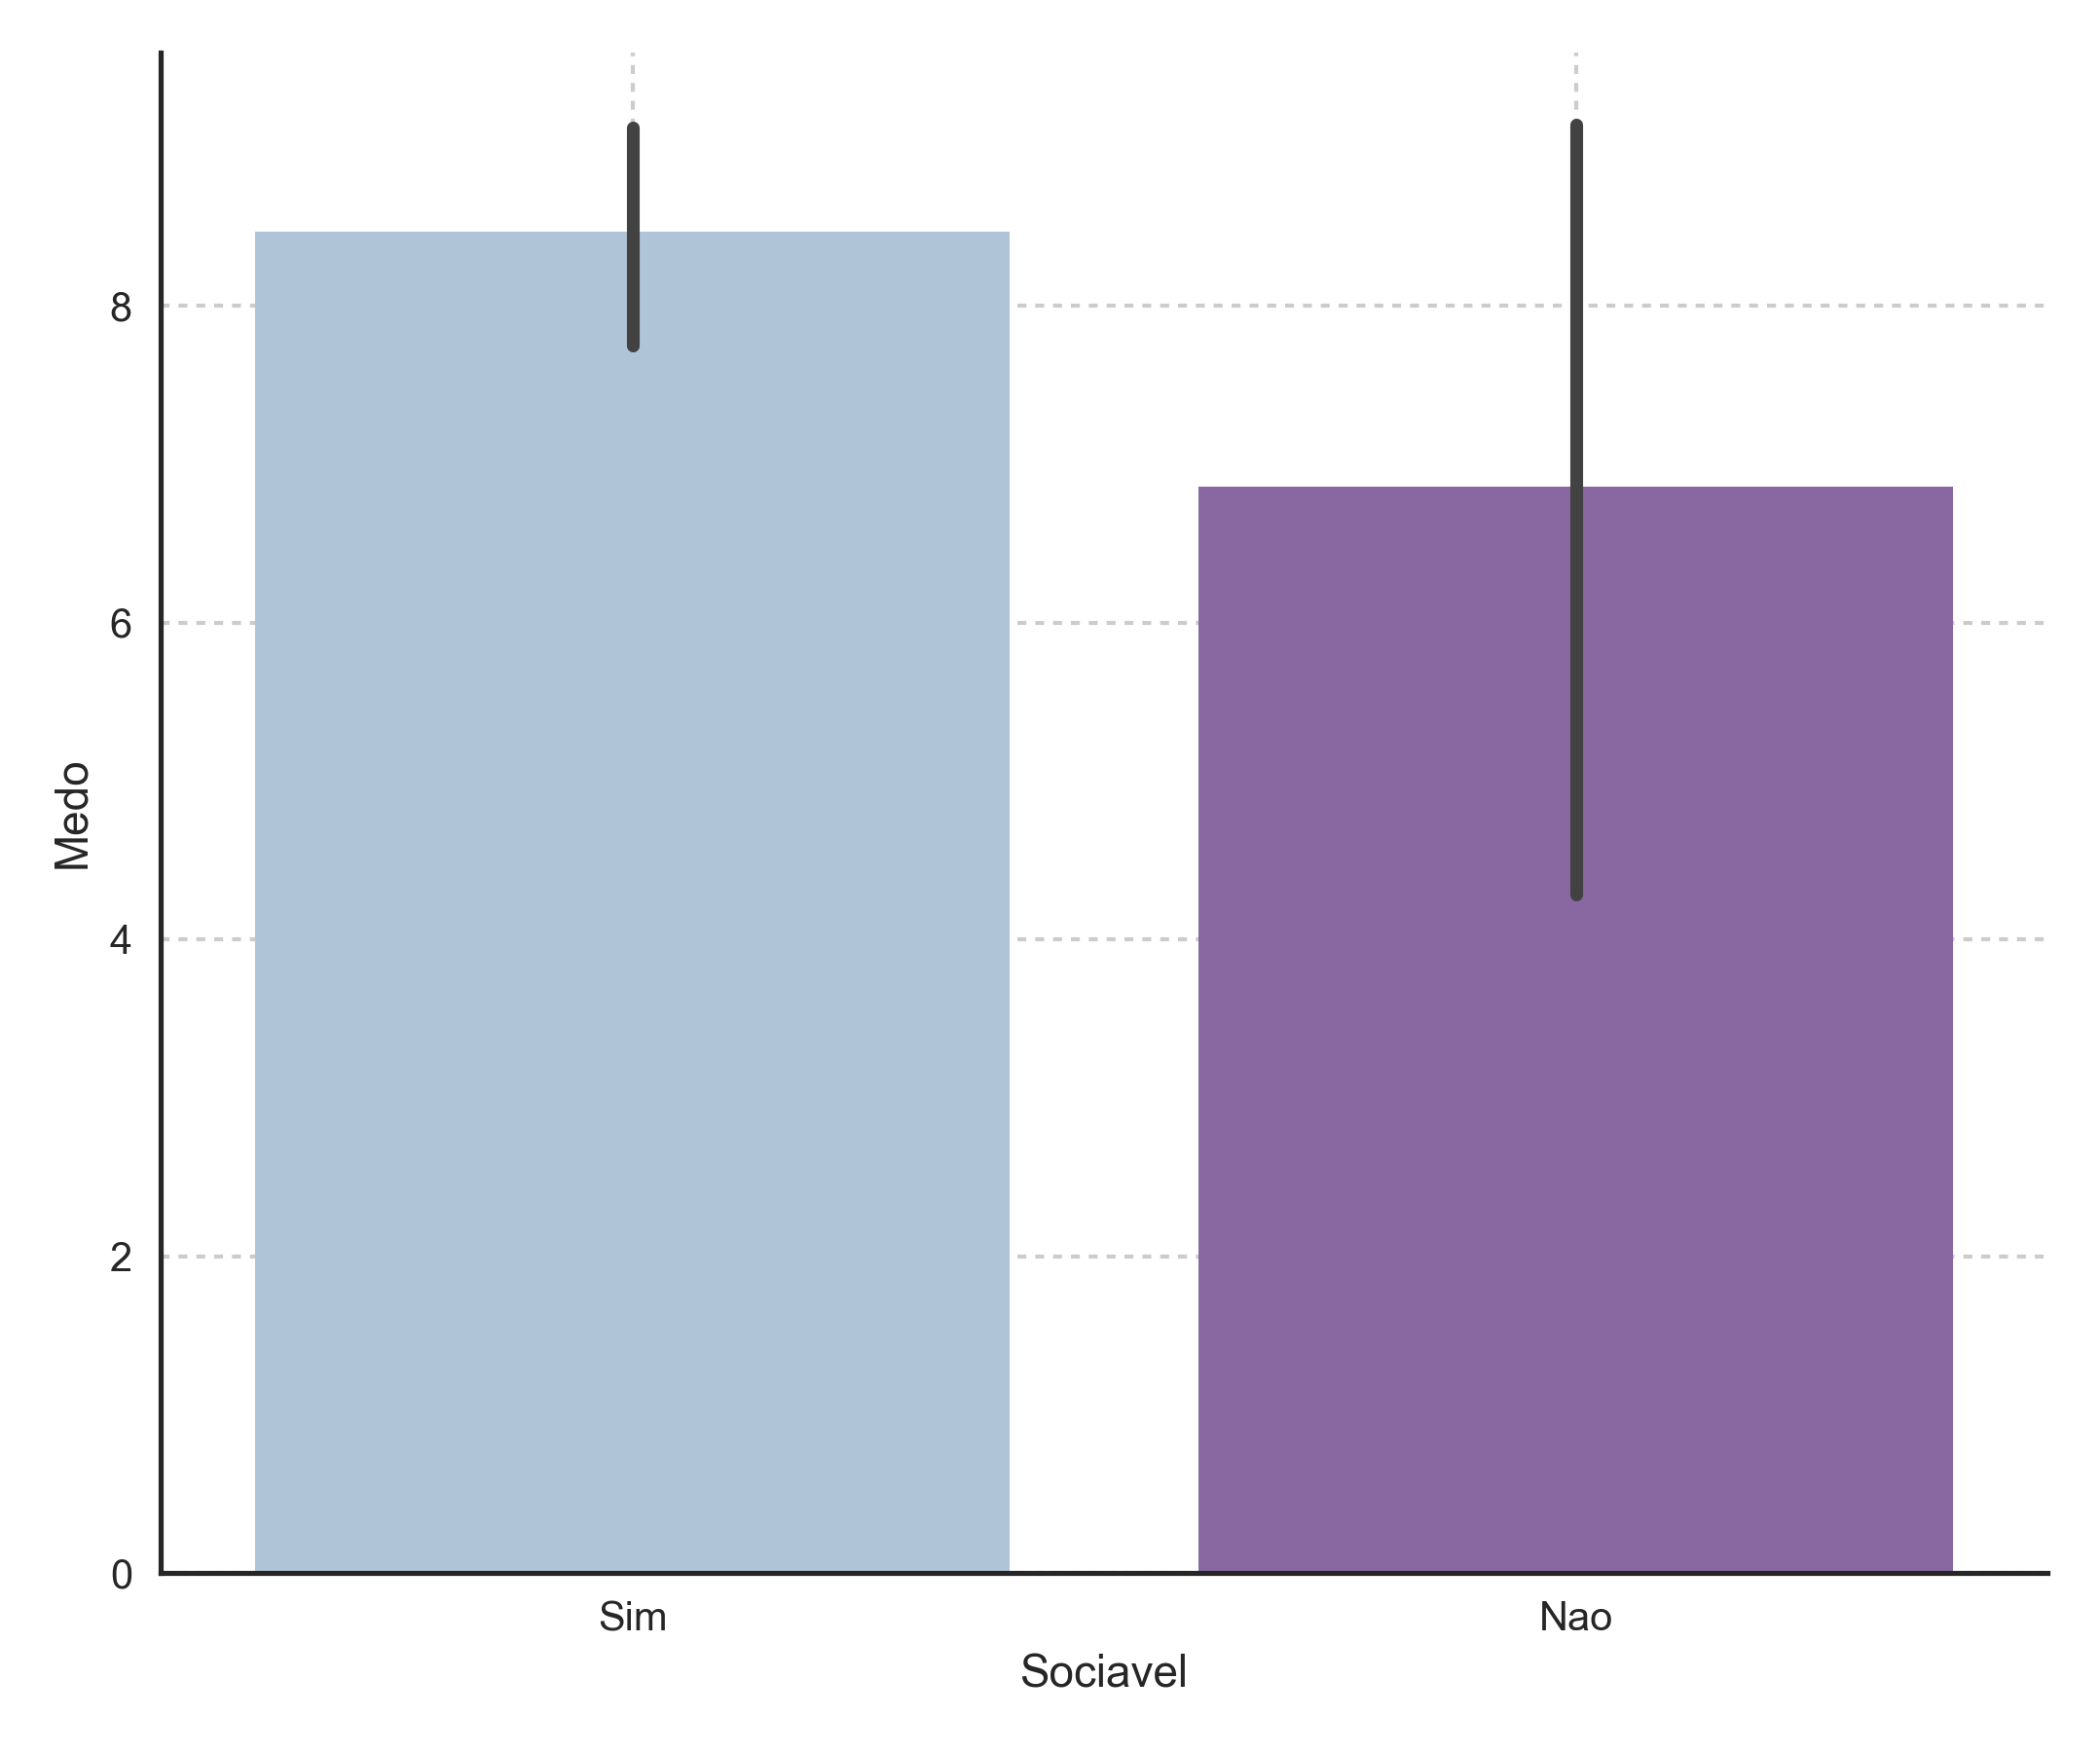
\includegraphics[width=\textwidth]{medo_sociavel.png}
		\smallcaption{Fonte: O autor.}
		\label{fig:medosociavel}
	\end{minipage}
\end{figure}

Após as análises gerais sobre as informações coletadas, é possível obter um grupo de perfis de usuários. Para obter os grupos de perfis, utilizou-se o algoritmo de agrupamento por similaridade QG-SIM. Foram testados três valores Q para determinar os grupos, 0.6, 0.7 e 0.8 de similaridade. O valor 0.6 apresentou 3 grupos, porém um dos grupos ficou com 90\% dos perfis e ou outros 10\% foram distribuídos para os demais grupos. Essa opção gerou um resultado muito generalizado e que não condiz com os perfis que realizaram os testes.

Quando aplicado o valor de 0.8 de similaridade para o algoritmo, 7 grupos foram encontrados. Os grupos ficaram bem específicos, sendo que 4 dos 7 grupos eram compostos por apenas 1 pessoa. Dessa maneira, é possível identificar que o resultado gerado é muito especializado e provavelmente a partir de ponto cada vez mais grupos com uma pessoa serão encontrados. Esse não é o objetivo da técnica de Personas. Então este resultado também foi desconsiderado.

Um valor intermediário foi escolhido. O valor de 0.7 apresentou 5 grupos. Um grupo com 21 perfis, que resultou na Persona Joaquim. Um grupo com 7 pessoas para Persona Maria Eduarda. Outro grupo com 9 pessoas deu origem a Persona Alfredo. As outras duas Personas foram criadas com base em dois grupos de 1 pessoa. Apesar de serem formados por apenas 1 pessoa, algumas características foram totalmente descriminante. A Persona Manuel, por exemplo, não tem acesso, nem conta em redes sociais. E a Persona Danielo aplicou a nota positiva máxima em todas as situações de interação. Esses foram fatores decisivos para que esses perfis permanecessem isolados em um grupo cada um.

Cada perfil dentro dos grupos mantém uma consistência demográfica e também de opinião sobre os comportamentos e ações do robô. A seguir serão apresentadas em tabelas as informações dos perfis para algumas perguntas chaves do questionário de maneira sintetizada. As informações referentes a expectativa da pessoa com o robô em casa encontra-se na tabela~\ref{tab:expectativacasa}.

\begin{table}[!ht]
	\caption{Expectativa do robô em casa dos perfis por Persona.}
	\label{tab:expectativacasa}
	\centering
	\begin{tabular}{c | c | c }
        \hline
        \multicolumn{3}{c}{Expectativa do robô em casa?} \\
        \hline
        Persona & Observação & Quantidade \\
        \hline
        \multirow{7}{*}{Joaquim} & Limpar a casa & 7 \\
        \hhline{~--}
        & Buscar objetos & 1 \\
        \hhline{~--}
        & Cuidar da segurança & 1 \\
        \hhline{~--}
        & Obediência & 4 \\
        \hhline{~--}
        & Afetividade & 4 \\
        \hhline{~--}
        & Naturalidade & 3 \\
        \hhline{~--}
        & Respeito & 3 \\
        \hline
        \multirow{3}{*}{Maria Eduarda} & Realizar tarefas domésticas & 5 \\
        \hhline{~--}
        & Dirigir o carro & 1 \\
        \hhline{~--}
        & Amigável & 1 \\
        \hline
        \multirow{4}{*}{Alfredo} & Realizar tarefas domésticas & 5 \\
        \hhline{~--}
        & Comandos de voz & 2 \\
        \hhline{~--}
        & Obediência & 2 \\
        \hline
        Danielo & Realizar tarefas domésticas & -- \\
        \hline
        Manuel & Atender necessidades & -- \\
        \hline
    \end{tabular}
    \smallcaption{Fonte: O autor.}
\end{table}

A pergunta da expectativa do robô em casa foi realizada antes da interação com o robô. Com base nas respostas pode-se perceber que as pessoas enxergam os robôs como ferramentas, antes de interagir e perceber do que os robôs são capazes. Em alguns casos, a mudança de opinião é nítida e será discutida mais a frente nessa seção. Outra pergunta realizada antes da interação com o robô é a expectativa em relação ao ambiente de trabalho. As respostas compiladas são apresentadas na tabela~\ref{tab:expectativatrabalho}.

\begin{table}[!ht]
	\caption{Expectativa do robô no ambiente de trabalho dos perfis por Persona.}
	\label{tab:expectativatrabalho}
	\centering
	\begin{tabular}{c | c | c }
        \hline
        \multicolumn{3}{c}{Expectativa do robô no ambiente de trabalho?} \\
        \hline
        Persona & Observação & Quantidade \\
        \hline
        \multirow{10}{*}{Joaquim} & Obediência & 4 \\
        \hhline{~--}
        & Realizar tarefas & 7 \\
        \hhline{~--}
        & Indiferente sobre o robô no trabalho & 1 \\
        \hhline{~--}
        & Eficiência nas atividades & 2 \\
        \hhline{~--}
        & Comunicação & 1 \\
        \hhline{~--}
        & Antecipar tarefas & 1 \\
        \hhline{~--}
        & Gerenciador de \emph{TODO List} & 1 \\
        \hhline{~--}
        & Otimizar processos & 1 \\
        \hhline{~--}
        & Seja sociável & 1 \\
        \hhline{~--}
        & Agir com naturalidade & 2 \\
        \hline
        \multirow{3}{*}{Maria Eduarda} & Realizar tarefas & 4 \\
        \hhline{~--}
        & Eficácia & 1 \\
        \hhline{~--}
        & Amigável & 1 \\
        \hline
        \multirow{3}{*}{Alfredo} & Realizar tarefas & 6 \\
        \hhline{~--}
        & Rápido & 1 \\
        \hhline{~--}
        & Obediência & 1 \\
        \hline
        Danielo & Executar tarefas repetitivas & -- \\
        \hline
        Manuel & Atender necessidades & -- \\
        \hline
    \end{tabular}
    \smallcaption{Fonte: O autor.}
\end{table}

Apesar da expectativa no trabalho ser a realização de tarefas, em linhas gerais, alguns outros pontos foram levantados. Comunicação, naturalidade, amigável, sociável e outros adjetivos voltados para convívio social começam a ganhar destaque em ambientes corporativos. As tabelas a seguir são de informações que foram coletadas após o experimento de interação social com o robô.
